\paragraph{Introduction:}In this chapter, we will present our contribution by describing the approach used and discussing the results of the performance of our models. The experiments described were also submitted for the ImageCLEF 2019 Tuberculosis severity scoring competition.  n addition, the work resulted in the submission of a conference paper. The ranking and the performance of the models resulted by the submissions to ImageCLEF 2019 SVR will be presented.

\paragraph{}
We proposed the system presented in Figure~\ref{fig:system}. The latter goes through two essential steps: input data pre-processing and learning a classification model. We will detail our proposed system in the following.
\begin{figure}[h!]
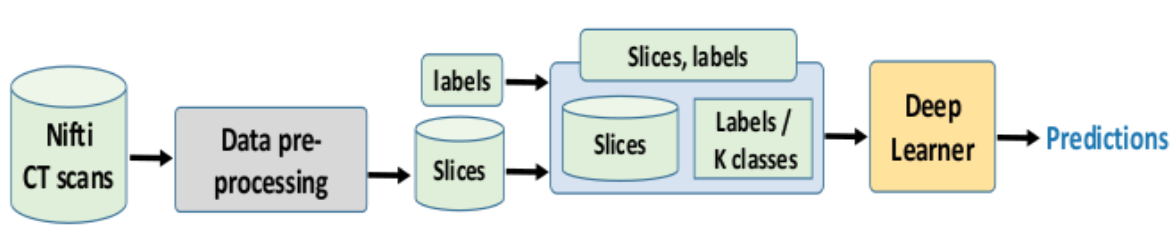
\includegraphics[width=\textwidth]{system.png}
\caption{The architecture of the overall proposed system} 
\label{fig:system}
\end{figure}

\section{Input data pre-processing}
\label{preprocess}
3D CT scans are provided in compressed Nifti format. Firstly, we decompress the files and extract the slices. In the end, we have three sets of slices corresponding to the three dimensions of the 3D image. For each dimension and for each Nifti image we obtain a number of slices ranging according to the dimension considered (512 images for the $Y$ and $X$ dimensions, from 40 to 250images for the $Z$ dimension).
\paragraph{}
The visual content of the images extracted from the different dimensions is not similar. Indeed, the images of each dimension are taken from a different view angle. We noticed from our experiments that the slices of the -Z- dimension give better results compared to the two others (X and Y). This is why we used in our work the Z-dimension. However, all steps can be applied to slices of any of the three dimensions.
\paragraph{}
After choosing the dimension to consider, we propose to filter the slices of each patient. Indeed, we can notice that many slices do not necessarily contain relevant information that could help to classify the samples due to their resemblance along the three dimensions. This is why we add a step to filter and select a number of slices per patient. For this, we propose two filtering approaches:
\begin{figure}[h!]
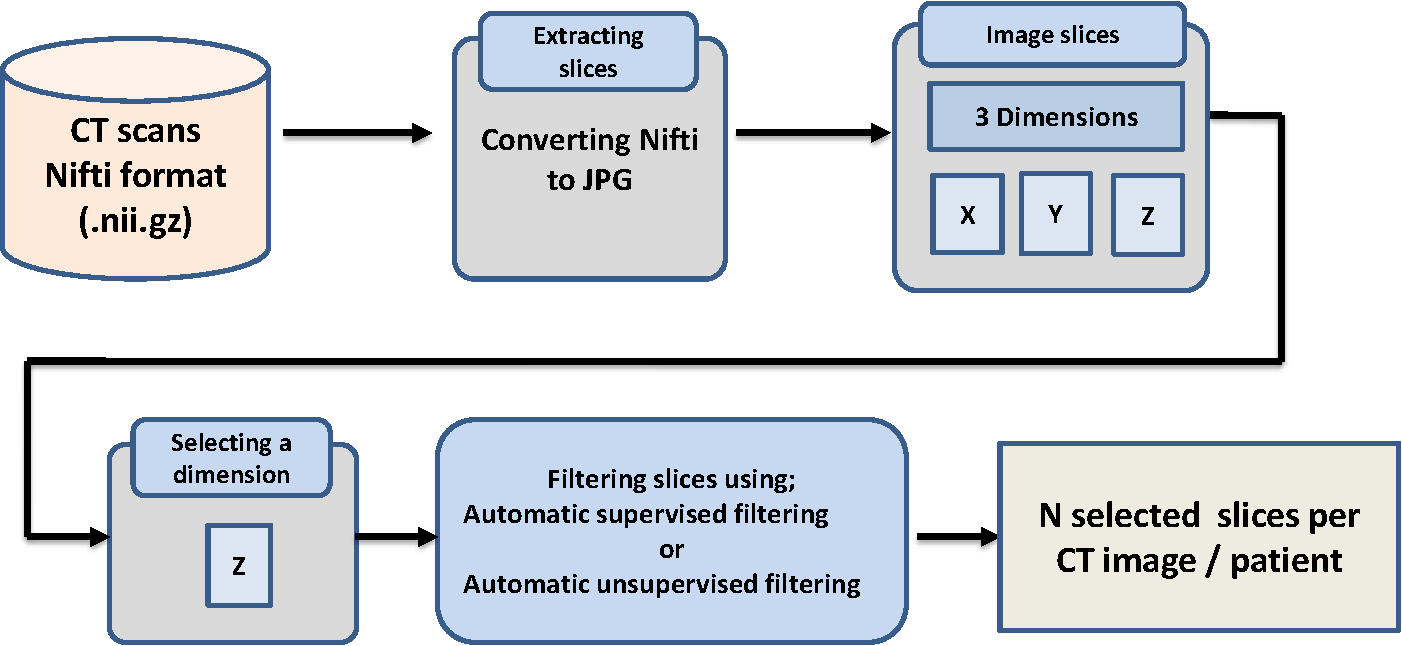
\includegraphics[width=\textwidth,height=6cm]{preprocess.pdf}
\caption{The architecture of the overall proposed system} 
\label{fig:preprocess}
\end{figure}
\paragraph{Automatic supervised filtering:}In this approach, we select a set of patients from each of the considered classes (the five degrees of severity for the SVR task). Then, a human expert selects for each patient, the slices likely to contain relevant information indicating the presence of Tuberculosis. The resulting set of slices constitutes a filtering group. Given a new patient, we compare each of its slices to the filtering group by calculating a distance measure:  a weighted sum of distances between the slice and those of the filtering group. We selected at the end $N$ slices that are judged to be the most similar to the filtering group. So, in the end, each patient is represented by the $N$ filtered slices instead of all its extracted images. We think that this would reduce the noise introduced by the consideration of all slices. We tested in our contributions the value N=10.

\paragraph{Automatic unsupervised filtering:}We noticed that there is usually a maximum of 50/60 slices visually informative. Since the slices are ordered, these most informative slices are usually at the center of the list. We propose then to keep only the $N$ middle ones. This is not optimal but we opted for this choice for a fully automatic and unsupervised approach. This choice can be improved by performing manual filtering with the intervention of a human expert, preferably with medical skills on TB disease.

Figure~\ref{fig:preprocess} summarizes the pre-processing steps.
\section{Deep learning models for CT image classification}
As a deep learner, we chose to use Resnet-50 architecture because of its good results in the context of the same problematic in last Tuberculosis task editions~\cite{sgeast17} and the google inceptionV3Resnet model. On the other hand, we developed a model that we called LungNet. We present more details about this model in the following section.

\paragraph{LungNet Deep Learner:}We proposed and developed our deep learner architecture for CT Image Analysis that we called LungNet. The input to the latter is an RGB image of size 119x119, followed by five convolutional layers and two fully connected layers. After each convolutional layer a ``relu" activation is applied followed by a local normalization and max pooling. the first, the second and third convolution blocks have dropout layers to reduce overfitting. The sigmoid activation function is applied to the output layer in order to predict values in the range of 0 to 1. Figure~\ref{fig:lungnet} illustrates the architecture of the Lungnet model.

\begin{figure}
%\vspace{-2cm}
\center
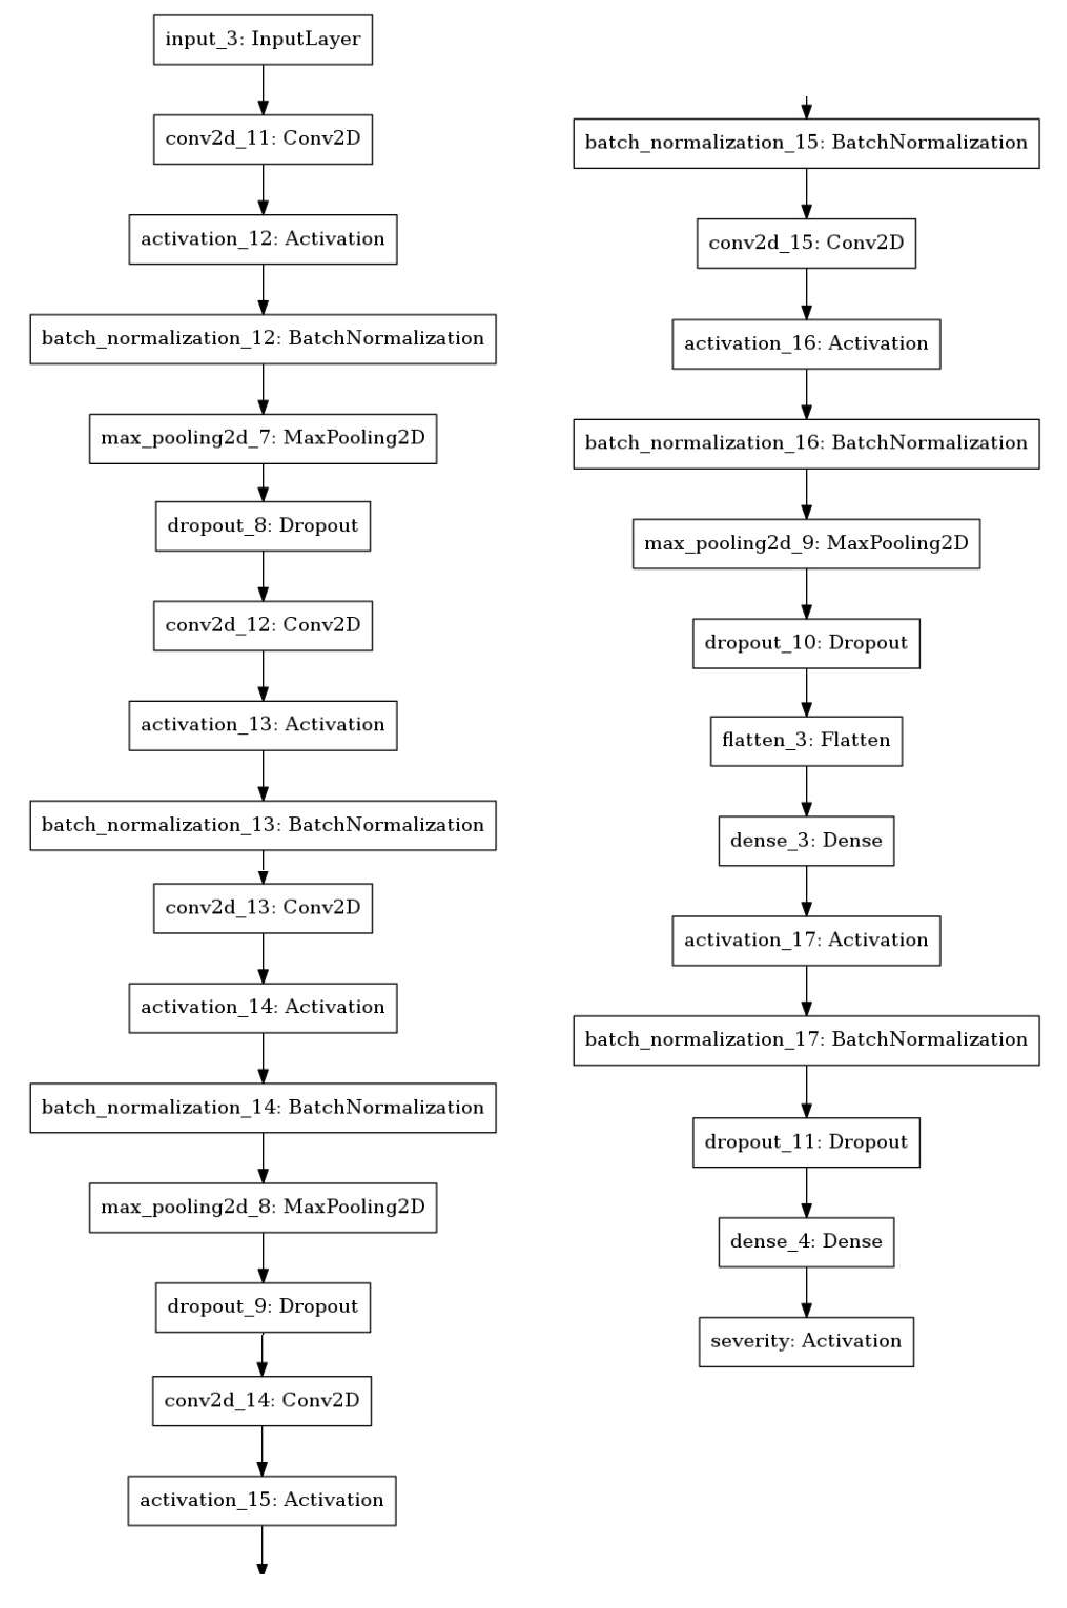
\includegraphics[width=10cm,height=10cm]{lungnet3.pdf}
\caption{The architecture of the LungNet Deep Learner} 
\label{fig:lungnet}
\end{figure}

\section{Experiments and results}
We describe in the following sections the different experiments performed for the SVR tasks. 

We used in our experimental work the following tools:
\begin{itemize}
\item med2image~\cite{med2image} for the conversion of nifti medical images to the classic Jpeg format;
\item Tensorflow frawework~\cite{tensorflow} and Keras library for deep learning;
\item scikit-learn~\cite{scikit-learn} library for testing several machine learning techniques.
\item tools and scripts developed by us~\cite{anouargit}.
\end{itemize}

We chose to use slices of the -Z- dimension because our experiments showed that they are more suitable than dimensions -X- and -Y- and got better results.

\subsection{Dataset}
The dataset used in the SVR task includes chest CT scans of TB patients along with some metadata regarding a set of 19 classes. 2 classes concern the SVR task, six other classes concern CTR task. The other values are considered as additional information regarding the patients that could be used as contextual information.

Table~\ref{tab1} summarizes the number of CT scans for train and test collections.

\begin{table}
\center
\caption{Dataset given for Tuberculosis SVR and CTR tasks~\cite{ImageCLEF19}.}
\label{tab1}
\begin{tabular}{|l|c|c|}
\cline{2-3}
\multicolumn{1}{}{}  &     \multicolumn{1}{|c|}{Train Collection}  &    \multicolumn{1}{|c|}{Test Collection}  \\
\hline
Number of patients             &    218                     &        117\\
\hline
\end{tabular}
\end{table}

The same dataset is given for the CTR task. The samples are labeled regarding eight main target classes: 
\begin{enumerate}
\item Target classes for SVR Task:
\begin{enumerate}
\item SVR\_severity (binary class : HIGH and LOW). Another label called md\_Severity is given (Five discrete values ranging from 1 to 5). We remind that values of md\_Severity (1, 2 and 3) belong to the ``HIGH" Severity class. The other two values (4 and 5) correspond to the ``LOW" Severity class.
\end{enumerate}
\end{enumerate}
\subsection{Experimental protocol}

We used the train collection provided by the organizers and we split it into two sub-collections: training and validation sets. The performed experiments are described below:
\begin{itemize}

\item \textbf{Resnet} : results of resnet50 deep learner trained on 50\% of data. Each patient was represented by 50 slices filtered using the automatic unsupervised filtering approach that was described in section~\ref{preprocess};

\item \textbf{Lungnet} : results of LungNet deep learner trained on 80\% of data. Each patient was represented by 10 slices filtered using the automatic supervised filtering approach that was described in section~\ref{preprocess};

\item \textbf{InceptionV3Resnet} : results of InceptionV3Resnet deep learner trained on 80\% of data. Each patient was represented by 50 slices filtered using the automatic unsupervised filtering approach that was described in section~\ref{preprocess};
\end{itemize}

In the case of Resnet50 and InceptionV3Resnet models, a hierarchical classification problem was considered.whereas, in the case of LungNet model, it was a direct binary classification.
\paragraph{Hierarchical classification:}Firstly, the probabilities of the 5 classes were generated by the model for n slice of the patient's CT scan. We will end up with a list of arrays holding the 5 class probabilities for each n slice. Then, an Argmax function is applied to each probability array to get the highly predicted class for each slice. This will result in a vector of values that represent the highly predicted class for each slice. we then choose the class that has the highest occurrence to be qualified as an elected class. The final step is to choose from the probability arrays list, the arrays that have the same argmax value as the elected class. Then, a column-wise mean is calculated for the list of elected arrays, resulting in a mean array of probabilities. Summing up the probabilities of 1st, 2nd and 3rd classes is what we considered as the probability of High severity class.
\paragraph{Binary classification:}The model was designed and trained to predict the probability of High severity class directly.

Our tools and scripts used in our experiments are accessible in~\cite{anouargit}.

\subsection{Results}

Table \ref{rsrs} shows the results in terms of AUC and accuracy obtained by our experiments on the evaluation performed by the ImageCLEF committee on test collection and our validation data.
\begin{table}
\center
\begin{tabular}{|l|l|l|l|l|l|l|}
\hline
          & \multicolumn{2}{l|}{Accuracy} & \multicolumn{2}{l|}{AUC} & \multicolumn{2}{l|}{Ranking}                                         \\ \hline
          & Validation      & Test        & Validation    & Test     & \multicolumn{2}{l|}{} \\ \hline
\textbf{Resnet50}  & 0.6300            & 0.6154      & 0.3400          & 0.6510   & \multicolumn{2}{l|}{22}                                              \\ \hline
\textbf{LungNet}   & 0.5220           & 0.6103      & 0.5260         & 0.5983   & \multicolumn{2}{l|}{33}                                              \\ \hline
\textbf{InceptionV3Resnet} & 0.5000        & 0.4701      & 0.4431         & 0.4933   & \multicolumn{2}{l|}{ 48} \\ \hline

\end{tabular}
\caption{Results on validation data and test set for SVR task (ImageClef submissions)}
\label{rsrs}
\end{table}
\newpage
\textbf{Confusion matrices:}
\begin{figure}[h!]
\centering
  \begin{subfigure}[b]{0.4\linewidth}
    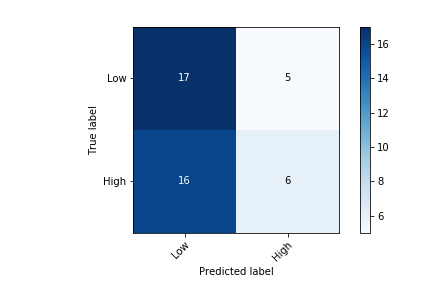
\includegraphics[width=\linewidth]{svr_lungnet_confusion_matrix.png}
    \caption{High-Low classes}
  \end{subfigure}
\label{lungnet_conf_mat}
\caption{Lungnet validation confusion matrix }
\end{figure}

\begin{figure}[h!]
\centering
  \begin{subfigure}[b]{0.4\linewidth}
    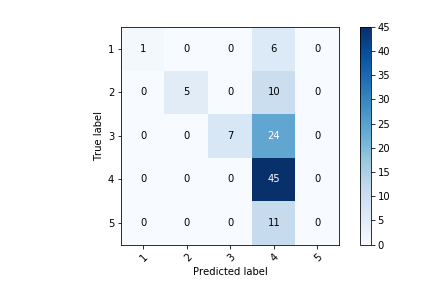
\includegraphics[width=\linewidth]{resnet_confusion_matrix.png}
    \caption{5-degrees classes}
  \end{subfigure}
  \begin{subfigure}[b]{0.4\linewidth}
    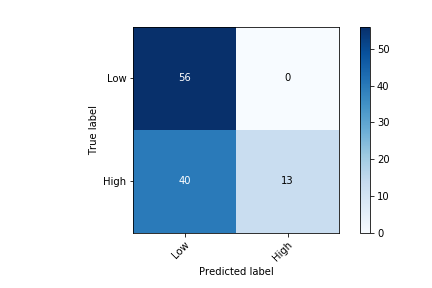
\includegraphics[width=\linewidth]{resnet_confusion_matrix_high_low.png}
    \caption{High-Low classes}
  \end{subfigure}
\label{resnet_conf_mat}
\caption{Resnet validation confusion matrices }
\end{figure}

\begin{figure}[h!]
\centering
  \begin{subfigure}[b]{0.4\linewidth}
    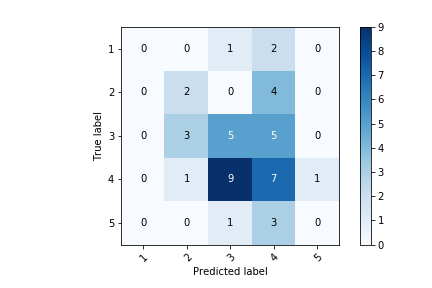
\includegraphics[width=\linewidth]{inceptionResnet_confusion_matrix_5_classes.png}
    \caption{5-degrees classes}
  \end{subfigure}
  \begin{subfigure}[b]{0.4\linewidth}
    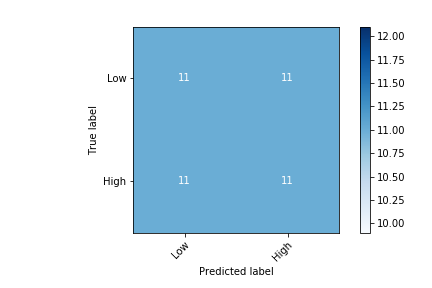
\includegraphics[width=\linewidth]{inceptionResnet_confusion_matrix_high_low.png}
    \caption{High-Low classes}
  \end{subfigure}
\label{InceptionV3Resnet_conf_mat}
\caption{InceptionV3Resnet validation confusion matrices }
\end{figure}
\newpage
\paragraph{}
The Resnet50 model got the best accuracy in validation and test datasets, followed by our developed model Lungnet with a small difference in term of test accuracy. the two models have outperformed the InceptionV3Resnet model. It is important to state that the LungNet model is a way smaller model than the resnet50 and InceptionV3Resnet and has been trained on less data than both models and yet achieved good results compared to those achieved by the other models. it would be interesting to see the performance of the Lungnet model after training it on  50 slices in order to make a detailed comparison with the perform of the other two models.\ref{fig:ranking} illustrates the ranking of the participating teams of the SVR task in terms of AUC and accuracy. We believe that our models could give better results after a more applying advanced data preprocessing including the use of masks, samples selection and data augmentation.
\begin{figure}[h!]
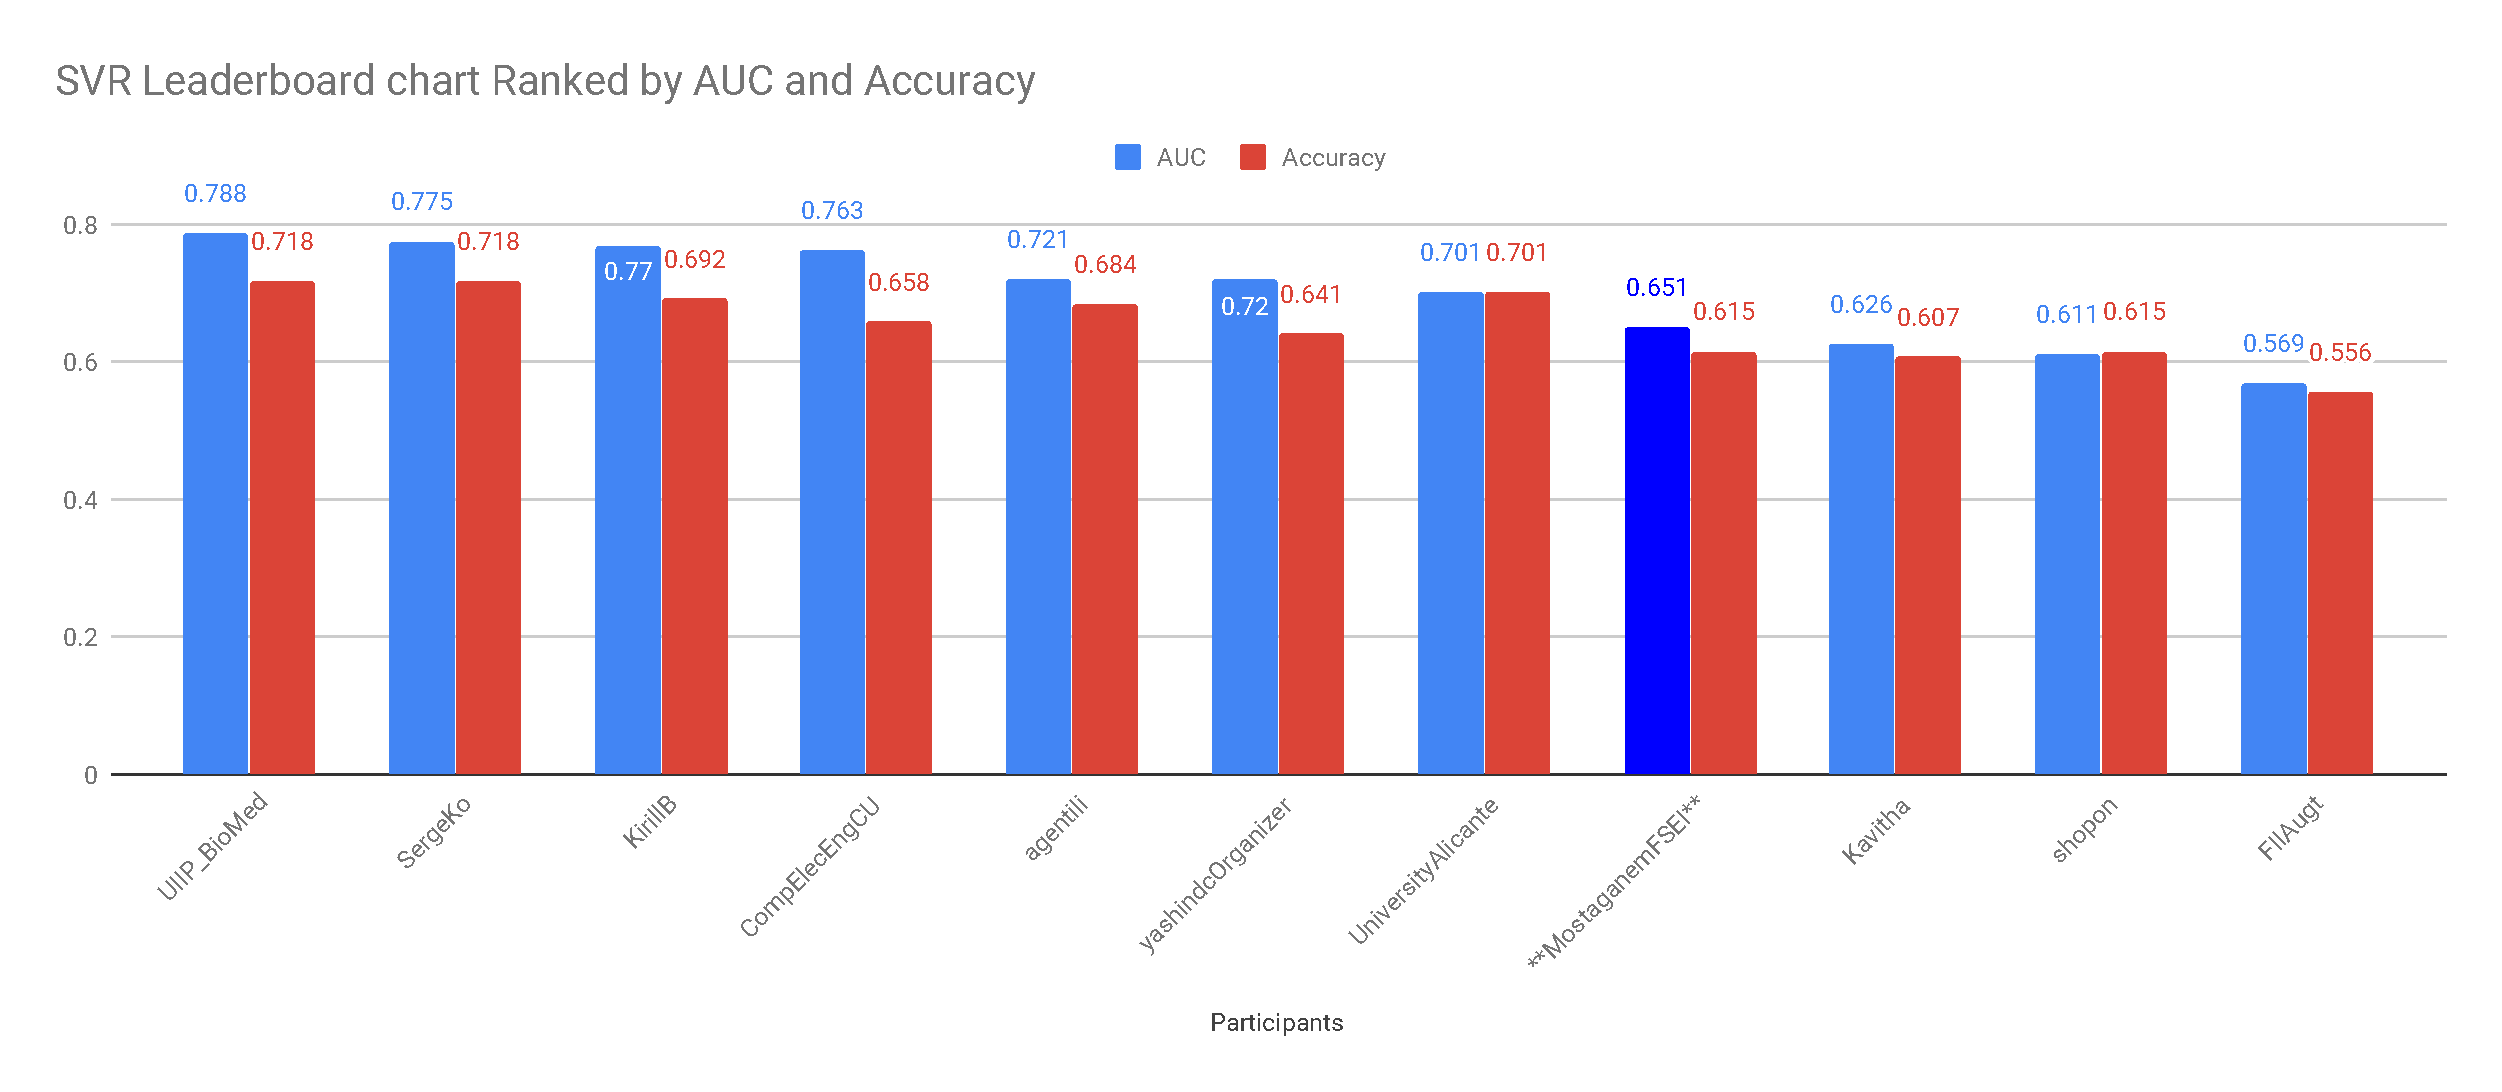
\includegraphics[width=\textwidth]{ranking.pdf}
\caption{Ranking of SVR task participants } 
\label{fig:ranking}
\end{figure}

\section{Conclusion}
\paragraph{}
We have described in this chapter our experiments of making a machine learning model to score the severity of a Tuberculosis case from a patient's CT scan and presented our participation submissions results in the SVR task of ImageCLEFmed Tuberculosis 2019. We proposed to use deep learner after preprocessing the CT scans in order to perform classification. We used for that, a Resnet-50, inceptionV3Resnet, and our proposed Lungnet architecture. Although our proposals had not been the best, the results obtained showed that these approaches could be much more efficient and give more interesting results if it is applied in an optimized way which includes advanced data-processing and the involvement of expert radiologists.
\paragraph{}
As perspectives, we plan to adopt enrichment strategies and learning samples selection. In addition, we noticed during the sub-sampling of our data that the deletion or addition of some samples had an impact on the results. On the other hand, filtering slices in an optimized way is a key idea that could further improve system performance. Furthermore, we noticed in our experiments that there is a difference in terms of precision achieved for each studied class. Indeed, some classes are more difficult to identify than others. This is also an interesting track to study. The use of masks and tracking the visual contents of the lungs could also be a good trail to explore.